\section{Kết quả thực nghiệm}

\subsection{Biểu đồ quá trình học (Learning Curves)}

\subsubsection{Epoch Curves - SGD Classifier}

SGD Classifier được huấn luyện bằng \texttt{partial\_fit} qua 20 epochs, cho phép ghi nhận Loss và Accuracy trên tập Train và Validation theo từng epoch (Hình~\ref{fig:sgd_epoch}).

\begin{figure}[H]
\centering
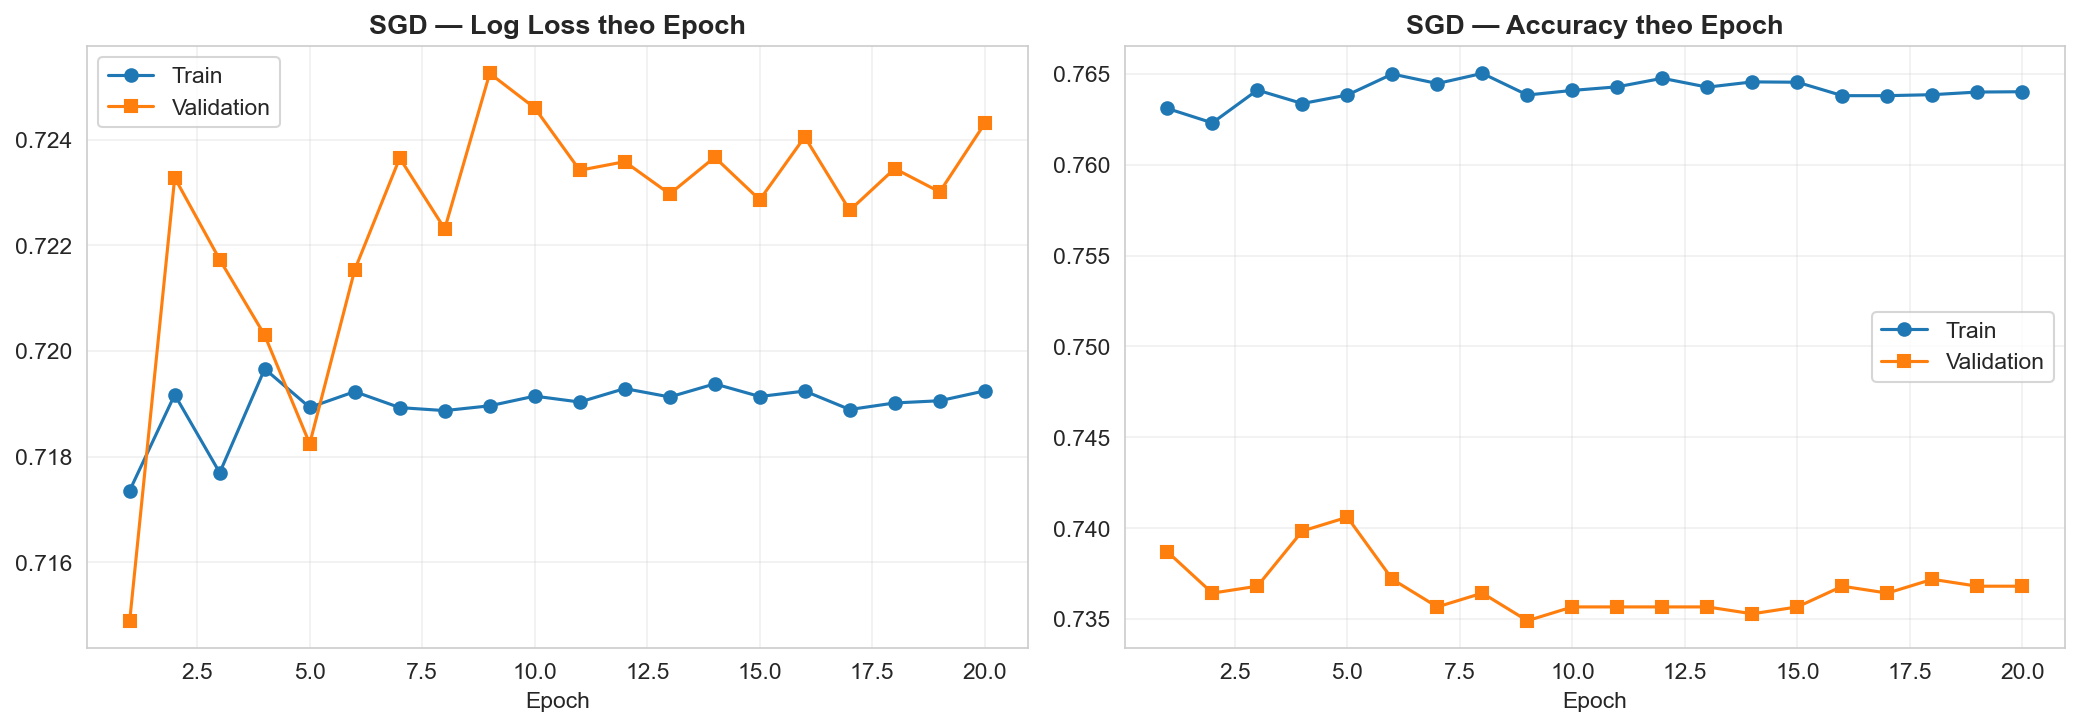
\includegraphics[width=0.85\textwidth]{figures/sgd_epoch_curves.png}
\caption{Biểu đồ Loss và Accuracy theo epoch của SGD Classifier trên tập Train và Validation}
\label{fig:sgd_epoch}
\end{figure}

\textbf{Nhận xét:} Mô hình hội tụ nhanh sau 3--5 epochs đầu tiên. Train Loss và Val Loss dao động ổn định quanh 0.72, cho thấy mô hình không bị overfitting. Val Accuracy ổn định ở mức $\approx$0.74 với biên độ dao động nhỏ ($<$0.005). Khoảng cách giữa Train Loss và Val Loss rất nhỏ, xác nhận mô hình tuyến tính với regularization phù hợp.

\subsubsection{Epoch Curves - PhoBERT}

PhoBERT được huấn luyện 3 epochs trên GPU Tesla T4, với kết quả đánh giá sau mỗi epoch (Hình~\ref{fig:phobert_curves}).

\begin{figure}[H]
\centering
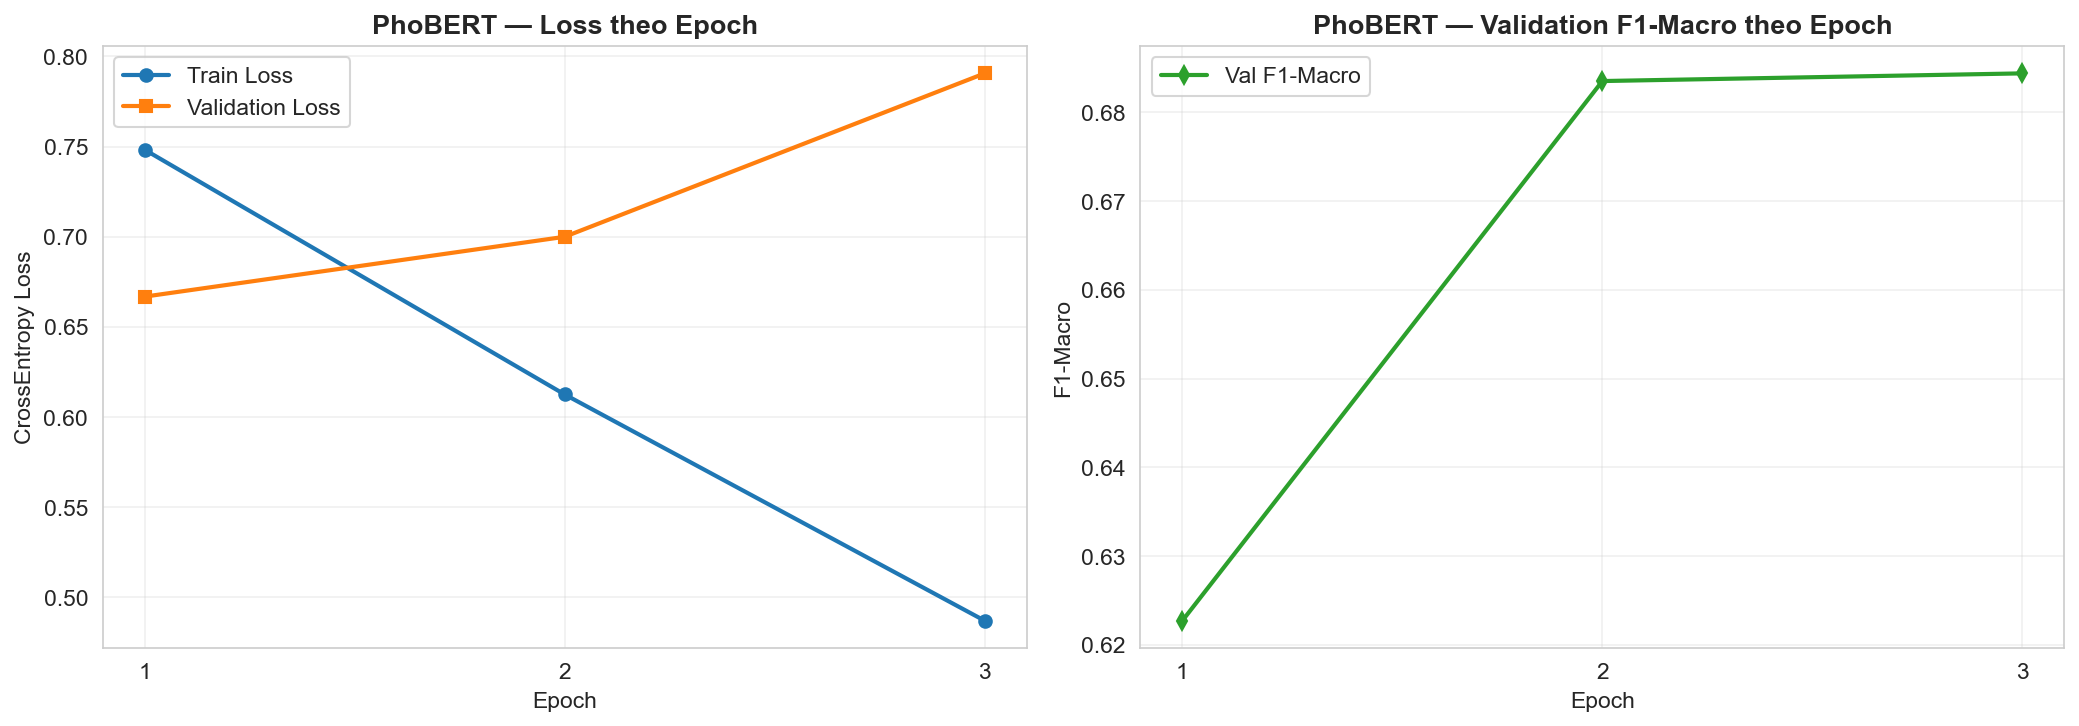
\includegraphics[width=0.85\textwidth]{figures/phobert_curves.png}
\caption{Biểu đồ Training Loss, Validation Loss, Accuracy và F1-macro theo epoch của PhoBERT}
\label{fig:phobert_curves}
\end{figure}

\textbf{Nhận xét:} Training Loss giảm đều qua 3 epochs (0.748 $\rightarrow$ 0.613 $\rightarrow$ 0.487). Validation Loss giảm ở epoch 1 (0.667) nhưng tăng nhẹ ở epoch 2--3 (0.700 $\rightarrow$ 0.791), cho thấy dấu hiệu \textbf{overfitting nhẹ} từ epoch 2. F1-macro tăng từ 0.623 lên 0.684 và ổn định. \texttt{load\_best\_model\_at\_end=True} đảm bảo mô hình tốt nhất (epoch 3, theo F1-macro) được giữ lại.

\subsubsection{Learning Curves theo Training Set Size}

Đối với các mô hình truyền thống (LR, SVM, RF), nhóm sử dụng \texttt{sklearn.model\_selection.learning\_curve()} để phân tích bias/variance qua F1-weighted trên 10 mức kích thước tập train (10\%--100\%), 3-fold CV (Hình~\ref{fig:lc_all}).

\begin{figure}[H]
\centering
\begin{subfigure}[b]{0.48\textwidth}
    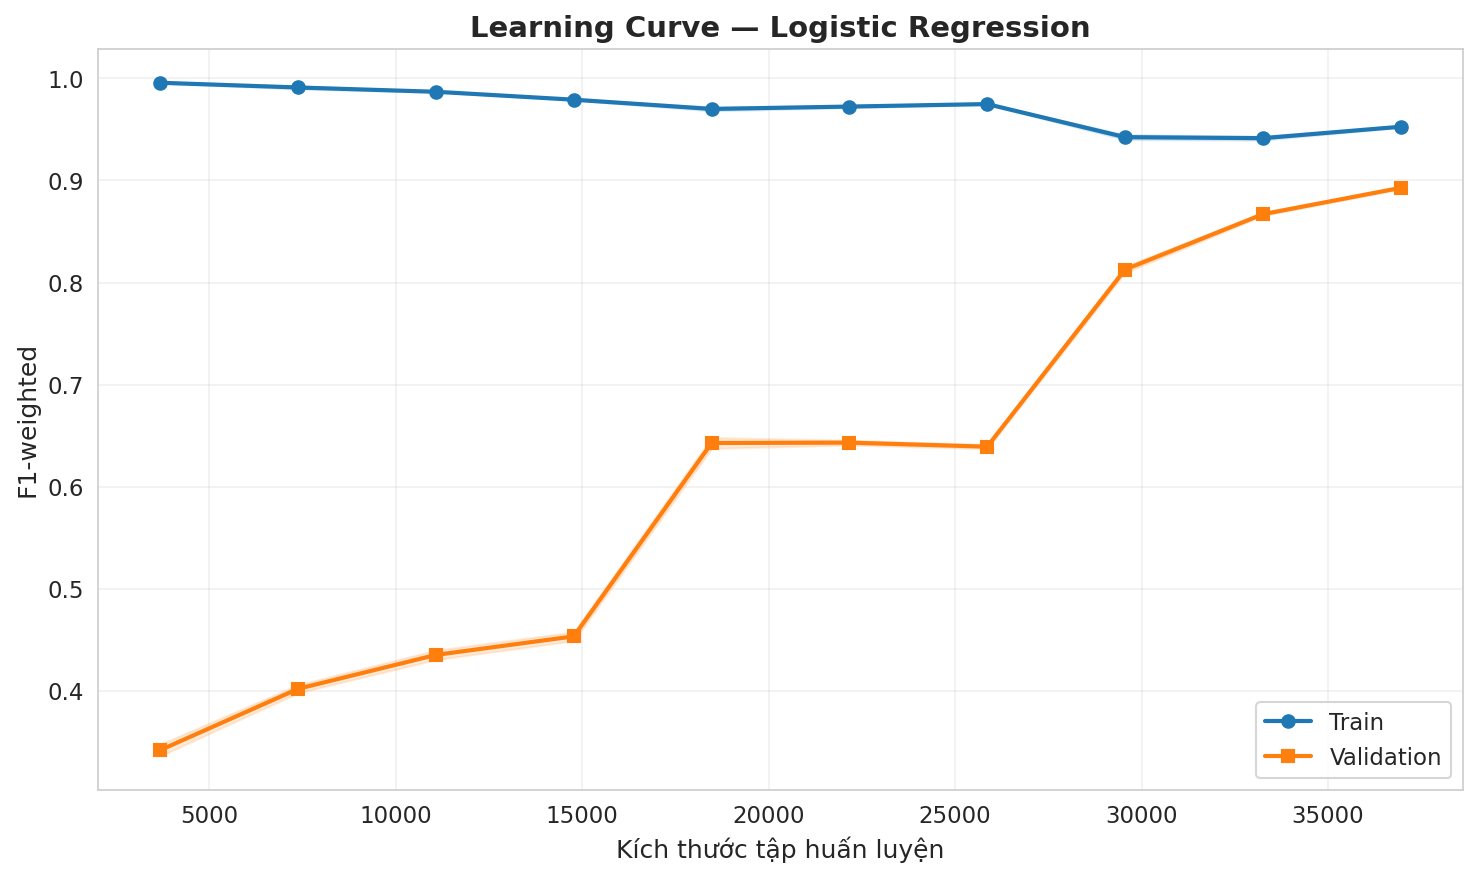
\includegraphics[width=\textwidth]{figures/lc_lr.png}
    \caption{Logistic Regression}
    \label{fig:lc_lr}
\end{subfigure}
\hfill
\begin{subfigure}[b]{0.48\textwidth}
    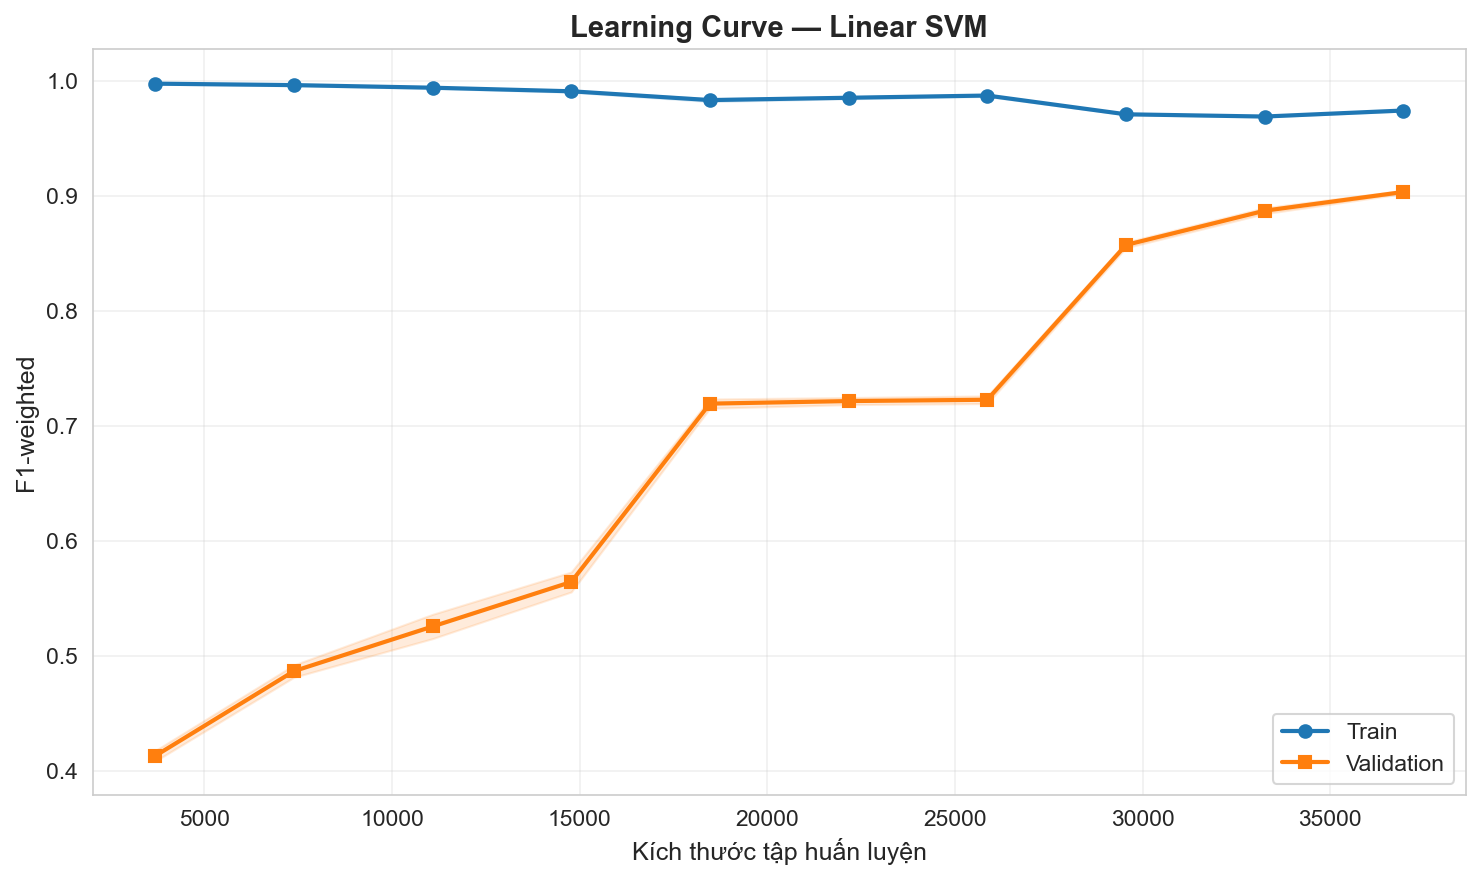
\includegraphics[width=\textwidth]{figures/lc_svm.png}
    \caption{Linear SVC}
    \label{fig:lc_svm}
\end{subfigure}

\vspace{0.5cm}
\begin{subfigure}[b]{0.48\textwidth}
    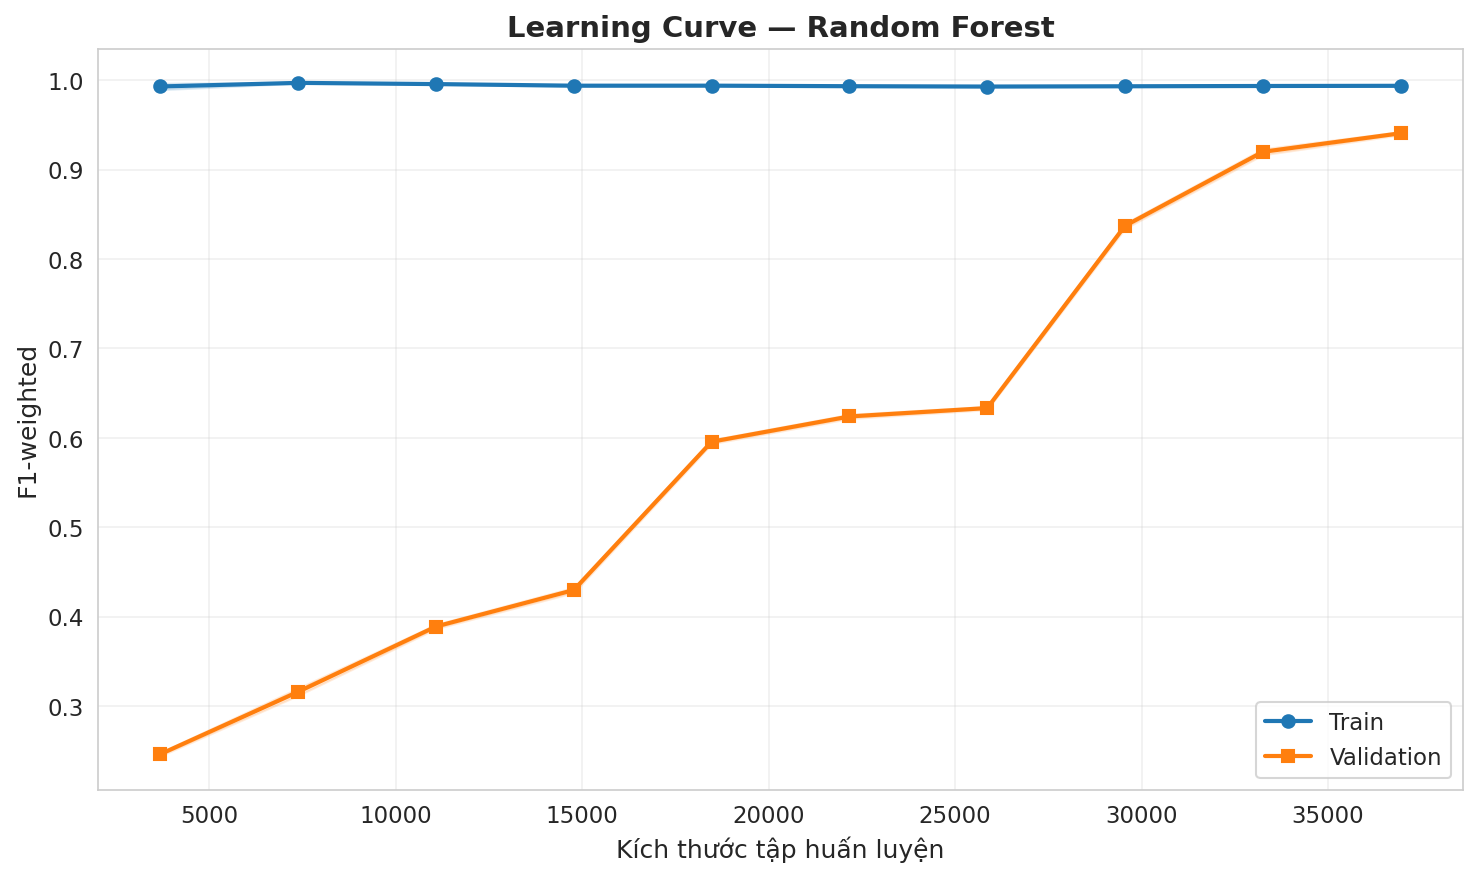
\includegraphics[width=\textwidth]{figures/lc_rf.png}
    \caption{Random Forest}
    \label{fig:lc_rf}
\end{subfigure}
\caption{Learning Curves (F1-weighted) theo kích thước tập huấn luyện}
\label{fig:lc_all}
\end{figure}

\textbf{Nhận xét:}
\begin{itemize}
    \item \textbf{Logistic Regression} (Hình~\ref{fig:lc_lr}): Train score giảm dần và Val score tăng dần khi tăng dữ liệu, hai đường tiệm cận nhau. Gap nhỏ $\Rightarrow$ low variance, mô hình ổn định.
    \item \textbf{Linear SVC} (Hình~\ref{fig:lc_svm}): Tương tự LR, hội tụ tốt. Gap giữa train và val nhỏ, cho thấy mô hình tuyến tính phù hợp với bài toán.
    \item \textbf{Random Forest} (Hình~\ref{fig:lc_rf}): Train score luôn rất cao ($\approx$1.0) trong khi Val score thấp hơn đáng kể ($\approx$0.94) $\Rightarrow$ dấu hiệu \textbf{overfitting} (high variance). Tuy nhiên val score vẫn tăng khi thêm dữ liệu, gợi ý mô hình có thể cải thiện nếu có thêm dữ liệu.
\end{itemize}

%------------------------------------------
\subsection{Đánh giá trên tập Test}

\subsubsection{Bảng so sánh tổng quan}

Bảng~\ref{tab:test_results} trình bày kết quả đánh giá trên tập Test (6{,}527 mẫu) cho tất cả 7 mô hình.

\begin{table}[H]
\centering
\caption{Kết quả đánh giá trên tập Test (sắp xếp theo F1-weighted)}
\label{tab:test_results}
\begin{tabular}{|l|c|c|c|c|c|}
\hline
\textbf{Mô hình} & \textbf{Accuracy} & \textbf{Precision\textsubscript{w}} & \textbf{Recall\textsubscript{w}} & \textbf{F1-weighted} & \textbf{F1-macro} \\
\hline
\textbf{PhoBERT-base-v2} & \textbf{0.8558} & \textbf{0.8733} & \textbf{0.8558} & \textbf{0.8637} & \textbf{0.6703} \\
Random Forest & 0.8079 & - & - & 0.8079 & - \\
Multinomial NB & 0.8068 & - & - & 0.8068 & - \\
Voting Ensemble & 0.7921 & - & - & 0.7921 & - \\
Logistic Regression & 0.7888 & - & - & 0.7889 & - \\
Linear SVC & 0.7888 & - & - & 0.7888 & - \\
SGD Classifier & 0.7746 & - & - & 0.7746 & - \\
\hline
\end{tabular}
\end{table}

\subsubsection{Classification Report - PhoBERT (mô hình tốt nhất)}

\begin{table}[H]
\centering
\caption{Classification Report của PhoBERT trên tập Test}
\label{tab:phobert_report}
\begin{tabular}{|l|c|c|c|c|}
\hline
\textbf{Lớp} & \textbf{Precision} & \textbf{Recall} & \textbf{F1-Score} & \textbf{Support} \\
\hline
CLEAN (0) & 0.95 & 0.90 & 0.93 & 5{,}406 \\
OFFENSIVE (1) & 0.40 & 0.52 & 0.45 & 440 \\
HATE (2) & 0.58 & 0.70 & 0.63 & 681 \\
\hline
\textbf{Weighted Avg} & \textbf{0.87} & \textbf{0.86} & \textbf{0.86} & \textbf{6{,}527} \\
\hline
\end{tabular}
\end{table}

%------------------------------------------
\subsection{Confusion Matrix}

Hình~\ref{fig:cm_all} hiển thị ma trận nhầm lẫn của hai mô hình đại diện: Voting Ensemble (mô hình truyền thống tốt nhất) và Logistic Regression (baseline).

\begin{figure}[H]
\centering
\begin{subfigure}[b]{0.48\textwidth}
    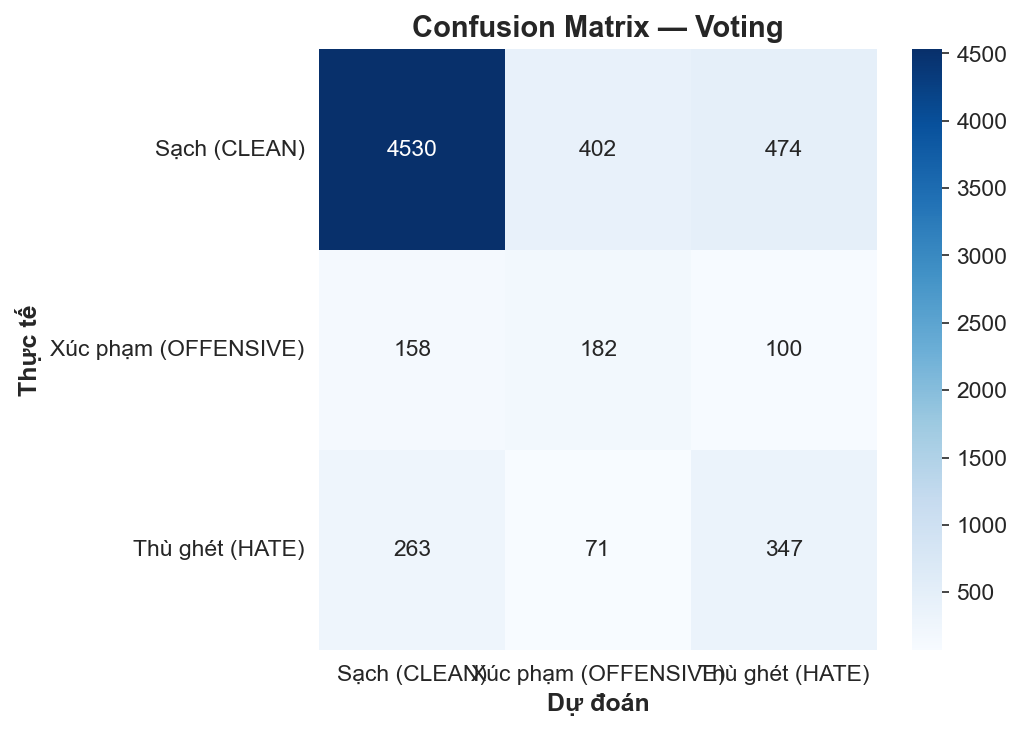
\includegraphics[width=\textwidth]{figures/cm_votingensemble.png}
    \caption{Voting Ensemble}
    \label{fig:cm_voting}
\end{subfigure}
\hfill
\begin{subfigure}[b]{0.48\textwidth}
    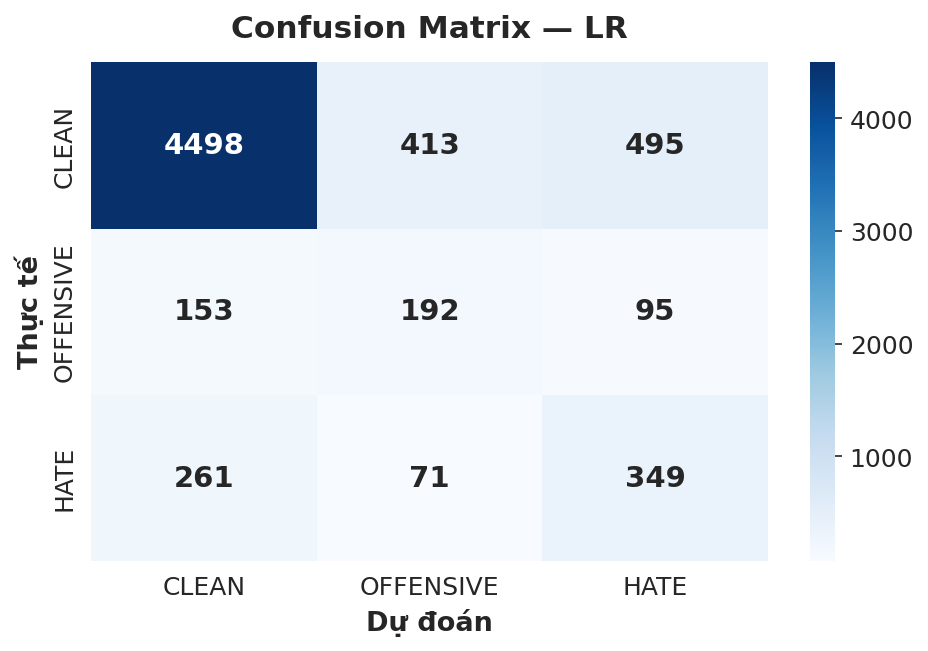
\includegraphics[width=\textwidth]{figures/cm_logisticregression.png}
    \caption{Logistic Regression}
    \label{fig:cm_lr}
\end{subfigure}
\caption{Ma trận nhầm lẫn trên tập Test}
\label{fig:cm_all}
\end{figure}

\textbf{Nhận xét:} Lớp CLEAN (nhãn 0) được phân loại chính xác nhất nhờ chiếm đa số dữ liệu. Lớp OFFENSIVE (nhãn 1) bị nhầm nhiều nhất - chủ yếu bị nhầm thành CLEAN (158 mẫu trong Voting Ensemble). Lớp HATE (nhãn 2) có recall tốt hơn OFFENSIVE nhờ bình luận thù ghét thường chứa từ ngữ mạnh, dễ phân biệt hơn.
